\section{Nixtla Neural Forecast NHITS}
{{\footnotesize
\begin{description}[labelwidth=5em, labelsep=1em, leftmargin=*, align=left, itemsep=0.3em, parsep=0em]
  \item[date:] 2023-06-01
  \item[version:] TODO
  \item[last\_updated:] 2025-06
  \item[expired:] unknown
  \item[valid:] yes
  \item[valid\_date:] TODO
  \item[url:] \href{https://github.com/Nixtla/neuralforecast}{https://github.com/Nixtla/neuralforecast}
  \item[doi:] TODO
  \item[domain:] Time-series; General ML
  \item[focus:] Official NHITS implementation for long-horizon time series forecasting
  \item[keywords:]
    - NHITS
    - long-horizon forecasting
    - neural interpolation
    - time-series
  \item[summary:] NHITS (Neural Hierarchical Interpolation for Time Series) is a state-of-the-art model that
improved accuracy by \textasciitilde{}25\% and reduced compute by 50x compared to Transformer baselines,
using hierarchical interpolation and multi-rate sampling :contentReference[oaicite:1]\{index=1\}.

  \item[licensing:] TODO
  \item[task\_types:]
    - Time-series forecasting
  \item[ai\_capability\_measured:]
    - Accuracy
    - compute efficiency for long series
  \item[metrics:]
    - RMSE
    - MAPE
  \item[models:]
    - NHITS
  \item[ml\_motif:]
    - Time-series
  \item[type:] Platform
  \item[ml\_task:]
    - Forecasting
  \item[solutions:] TODO
  \item[notes:] Official implementation in NeuralForecast, included since its AAAI 2023 release.

  \item[contact.name:] Kin G. Olivares (Nixtla)
  \item[contact.email:] unknown
  \item[datasets.links.name:] Standard forecast datasets, M4
  \item[results.links.name:] ChatGPT LLM
  \item[fair.reproducible:] Yes
  \item[fair.benchmark\_ready:] Yes
  \item[ratings.software.rating:] 0
  \item[ratings.software.reason:] Not analyzed.

  \item[ratings.specification.rating:] 7.0
  \item[ratings.specification.reason:] Primarily a visualization frontend; underlying benchmark definitions come from vLLM project.

  \item[ratings.dataset.rating:] 6.0
  \item[ratings.dataset.reason:] No traditional dataset; displays live or logged benchmark metrics.

  \item[ratings.metrics.rating:] 9.0
  \item[ratings.metrics.reason:] Live throughput, memory, latency, and TTFT displayed interactively; highly informative for performance analysis.

  \item[ratings.reference\_solution.rating:] 7.0
  \item[ratings.reference\_solution.reason:] Dashboard built on vLLM benchmarks but not itself a complete experiment package.

  \item[ratings.documentation.rating:] 8.0
  \item[ratings.documentation.reason:] Observable notebooks are intuitive; customization instructions are minimal but UI is self-explanatory.

  \item[id:] nixtla\_neural\_forecast\_nhits
  \item[Citations:] \cite{challu2023nhits}
  \item[Ratings:]
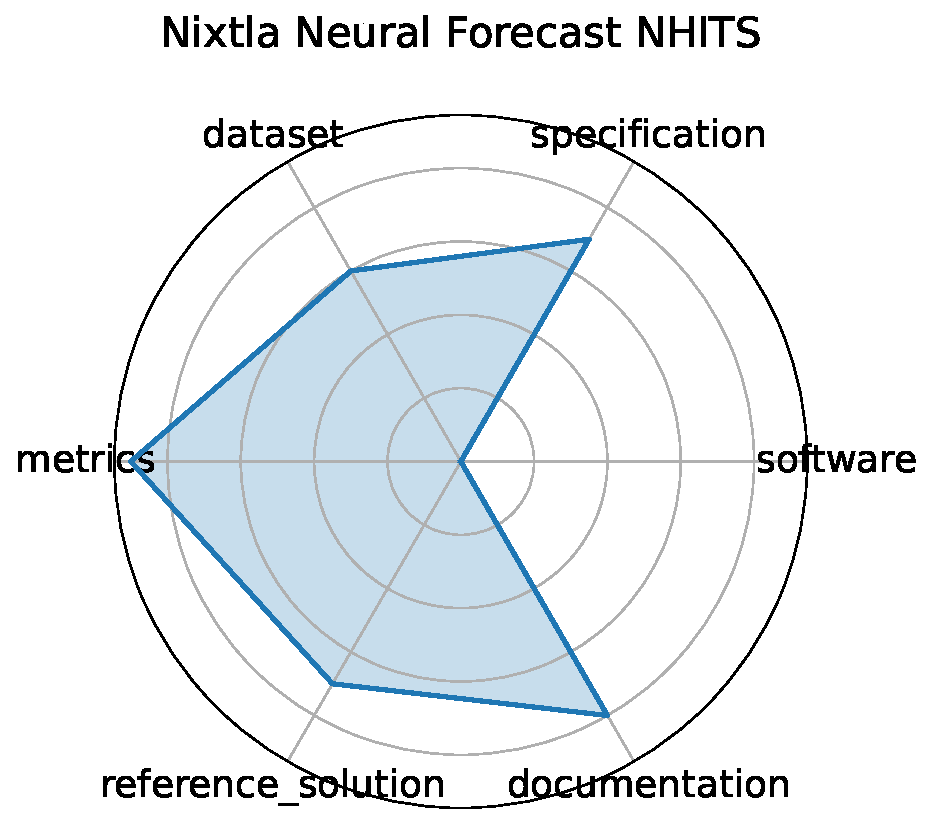
\includegraphics[width=0.2\textwidth]{nixtla_neural_forecast_nhits_radar.pdf}
\end{description}
}}
\clearpage